\documentclass{ximera}

%% The launch should somehow present a ``mystery'' for the students to
%% solve.  Moreover, it should lead them to the right path. Ideally if we
%% had a bright student working on the launch, they might even develop
%% the techniques from the lesson to solve teh problem. 
%% By the end of the lesson, the mystery is solved!

\title{From average rate of change to instantaneous rate of change}

\begin{document}
\begin{abstract}
The derivative computes the instantaneous rate of change. 
\end{abstract}
\maketitle

%% Here the idea is to be truthful, enthuastic, and narrow. We want a
%% SINGLE example. So for this prototype we could talk about all kinds
%% of rates of change, but lets refrain from this.


Let me tell you about something that is really awesome:
\href{http://en.wikipedia.org/wiki/Global_Positioning_System}{The
  Global Positioning System.} Seriously, this is a modern ``Wonder of
the World.'' With this system, the secrets of navigating our beautiful
blue sphere are no longer limited to an elite few. Instead we have
devices small enough to fit in our pockets, that cost as little as a
few meals, that can tell us where we are, and even \textit{how fast we
  are going.} Think about this, a mere $2000$ years ago, a GPS in the
right hands would have been powerful enough to change the course of
history!

While the details of how GPS works are fascinating, incorporating many
concepts from mathematics and physics, including
\href{relativisticEffectsInTheGlobalPositioningSystem.pdf}{Einstein's
  theory of relativity}, what we are most interested in is how a GPS
computes velocity from position.

The \textit{MOOCulus Team} recently took a road trip from Columbus
Ohio to Urbana-Champaign Illinois in the \textit{MOOCulus-Mobile}:
\begin{image}
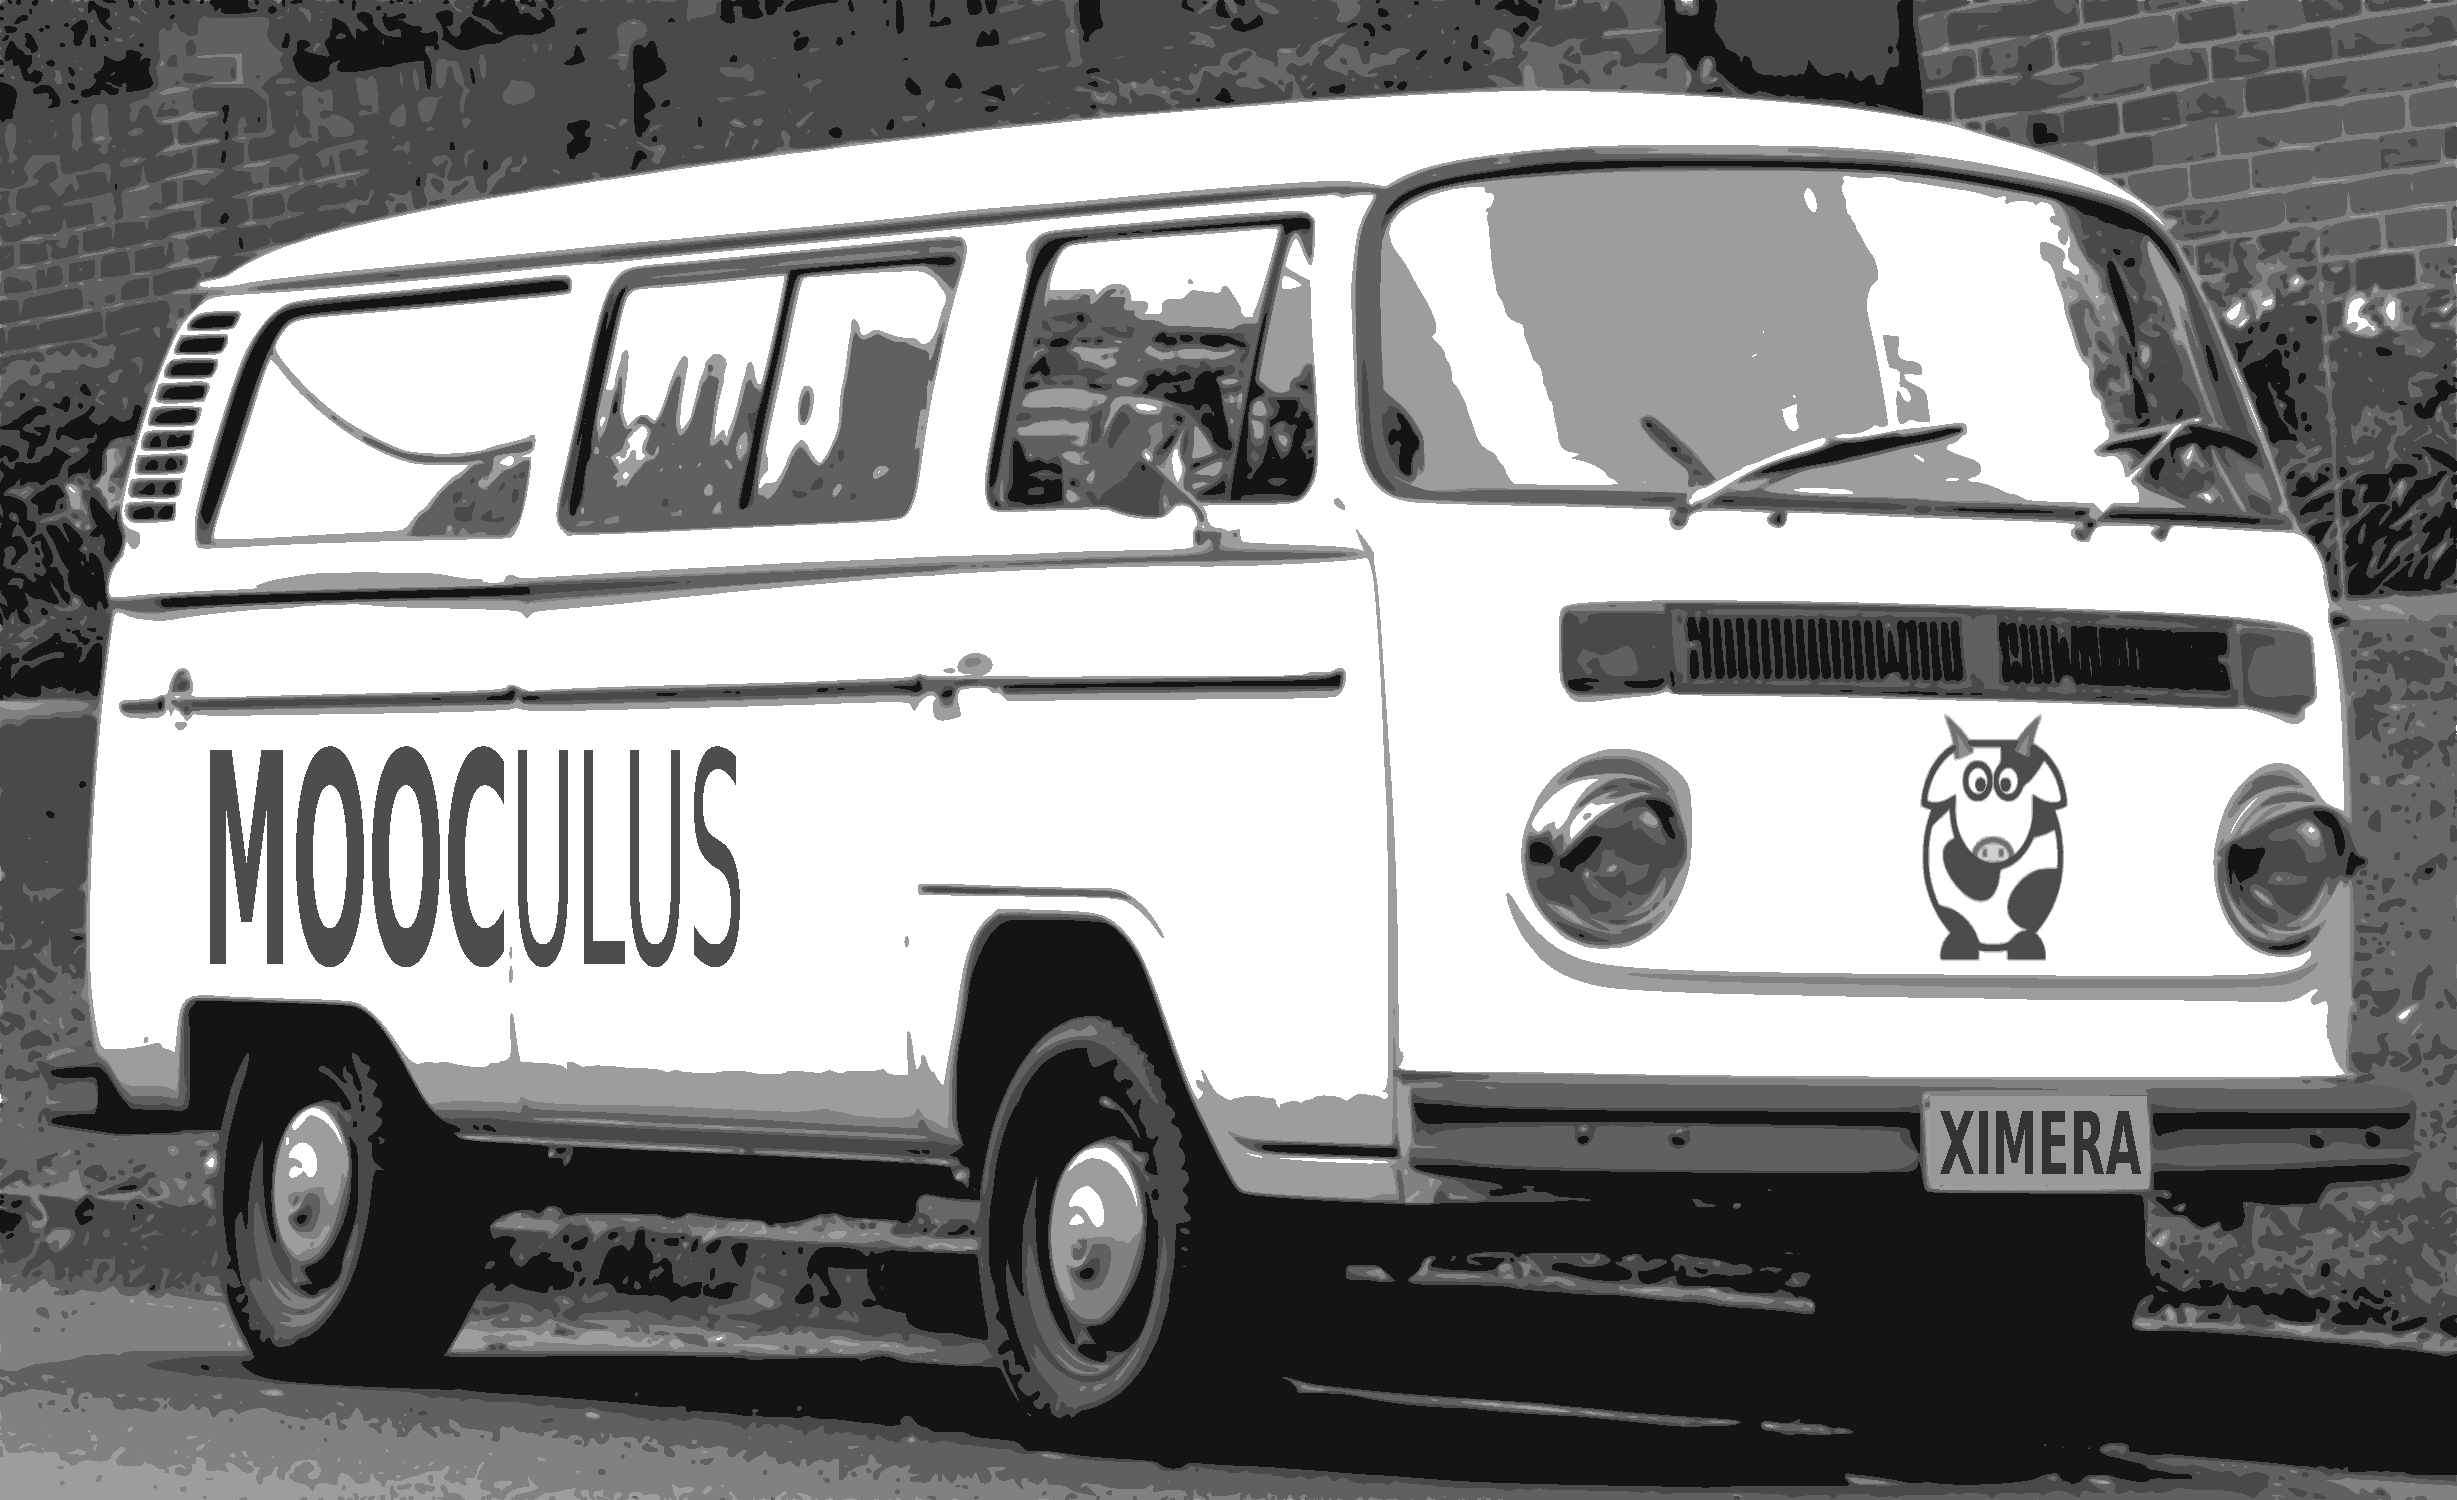
\includegraphics[width=3in]{mooculusMobile.pdf}
\end{image}
While the MOOCulus-Mobile might look pretty spiffy, it has some
quirks, in particular, it has no speedometer!  Never-to-be-flustered,
the MOOCulus team will just used their GPS to help them compute the
velocity. Let's see how. To do this, we need some
background. Urbana-Champaign is around $300$ miles dead West of
Columbus. The position of the MOOCulus-Mobile is roughly modeled by
\[
s(t) = 36t^2 -4.8t^3 \qquad\text{(miles West of Columbus)} %% note the model is wrong
\]
where $t$ is measured in hours. 

\begin{question} %% Here we are asking the student to think about context
What does $s(0)$ correspond to in terms of the context of our road
trip?
\begin{hint}
Remember $s(t)$ is position at time $t$.
\end{hint}
\begin{hint}
So $s(0)$ is how far you've gone after no time has passed. 
\end{hint}
\begin{multipleChoice}
  \choice[correct]{Our starting point, Columbus Ohio.}
  \choice{Our ending point, Urbana-Champaign Illinois.}
  \choice{Ann-Arbor Michigan, because the MOOCulus Team got lost.}
  \choice{There is no way to be certain.}
\end{multipleChoice}
\end{question}

\begin{question} %% Here we are asking the student to think about context
If $b$ corresponds to the time where $s(b) = 300$, what does $b$ mean
in terms of the context of our road trip?
\begin{hint}
Remember $s(t)$ is position at time $t$.
\end{hint}
\begin{hint}
So $s(b)=300$ is a statement relating time and position.  
\end{hint}
\begin{multipleChoice}
  \choice[correct]{$b$ is how many hours it takes the MOOCulus Team to travel to Urbana-Champaign.} 
  \choice{$b$ is the time the MOOCulus Team arrives after noon.}
  \choice{$b$ is the time the MOOCulus Team arrives after midnight.}
  \choice{There is no way to be certain.}
\end{multipleChoice}
\end{question}


\begin{question} %% A VERY important question
Consider again the function that roughly models the position of the
MOOCulus-Mobile
\[
s(t) = 36t^2 -4.8t^3
\]
Assuming the final destination is Urbana-Champaign Illinois, on what
domain does this model make sense?
\begin{hint}
  Plot $s(t)$ and choose the domain that make sense in the context of
  the problem.
\end{hint}
\end{question}

\begin{question}
  What is the average velocity for the MOOCulus-Mobile for the entire trip? 
\begin{hint}
Remember, 
\[
\text{distance} = \text{rate}\cdot\text{time}.
\]
\end{hint}
\begin{hint}
So, 
\[
\frac{\text{distance}}{\text{time}} = \text{rate}.
\]
\end{hint}
\end{question}

Now let's get a bit crazy, consider this interval:
\[
I_h = 
\begin{cases}
  [2+h,2]  & \text{if $-1<h<0$}, \\ %% note this is MORE correct than std books
  [2,2+h]  & \text{if $0<h<1$}.     %% in the content section, we can explain this in detail
\end{cases}
\]

\begin{question}
  What is this interval when $h = 0.3$?
\end{question}

\begin{question}
  What is the average velocity of the MOOCulus-Mobile on $I_h$ when $h =
  0.3$?
\end{question}

\begin{question}
  What is this interval when $h = -0.2$?
\end{question}

\begin{question}
  What is the average velocity of the MOOCulus-Mobile on $I_h$ when $h =
  -0.2$?
\end{question}

\begin{question}
  Write a formula that will compute the average velocity of the
  MOOCulus-Mobile at $t=2$ hours for all given values of $h$.
\end{question}

Computing average velocities for smaller, and smaller values of $h$ as
we did above is tedious. Nevertheless, this is exactly how a GPS
determines velocity from position! On the other hand, we are human
beings and have better things to do than just compute all day
long. What would really help us out is a formula.

\begin{question}
  Given a formula for position, say $s(t) = 36t^2 -4.8t^3$, how do we
  find a formula for velocity?  Think about the previous problem and
  what we have done previously in the course.
  \begin{freeResponse}
  \end{freeResponse} 
\end{question}

\begin{xarmaBoost}
  Write down at least \textbf{five} questions for this lecture. After
you have your questions, label them as ``Level 1,'' ``Level 2,'' or ``Level 3'' where:
\begin{description}
\item[Level 1] Means you know the answer, or know exactly how to do
  this problem.
\item[Level 2] Means you think you know how to do the problem, or will
  soon learn how to do the problem.
\item[Level 3] Means you have no idea how to do the problem.
\end{description}
\begin{freeResponse}
\end{freeResponse}
\end{xarmaBoost}

\end{document}
